\section{Ejercicio 2: Cálculos} 
		
\begin{enumerate}[1.]
	\item  En Power BI Desktop, haga clic en Datos en el panel de vistas en el lado izquierdo. En el panel Campos, haga clic en DimCustomer.  En la cinta Modelado, en el grupo Cálculos, haga clic en Nueva columna. En la barra de fórmulas, resalte Columna = y escriba:
	\\	
	\\
	\\IncomeStatus = IF (DimCustomer[YearlyIncome] < 25000, "Lower Income", \\
	  IF (AND(DimCustomer[YearlyIncome] >= 25000, DimCustomer[YearlyIncome] < 60000),\\
	  "Middle Income", \\
	   IF (AND(DimCustomer[YearlyIncome] >= 60000, DimCustomer[YearlyIncome] < 100000), \\
	"Higher Income", \\
	IF (DimCustomer[YearlyIncome] >= 100000, "Very High Income", "Other")))) \\

	\begin{center}
	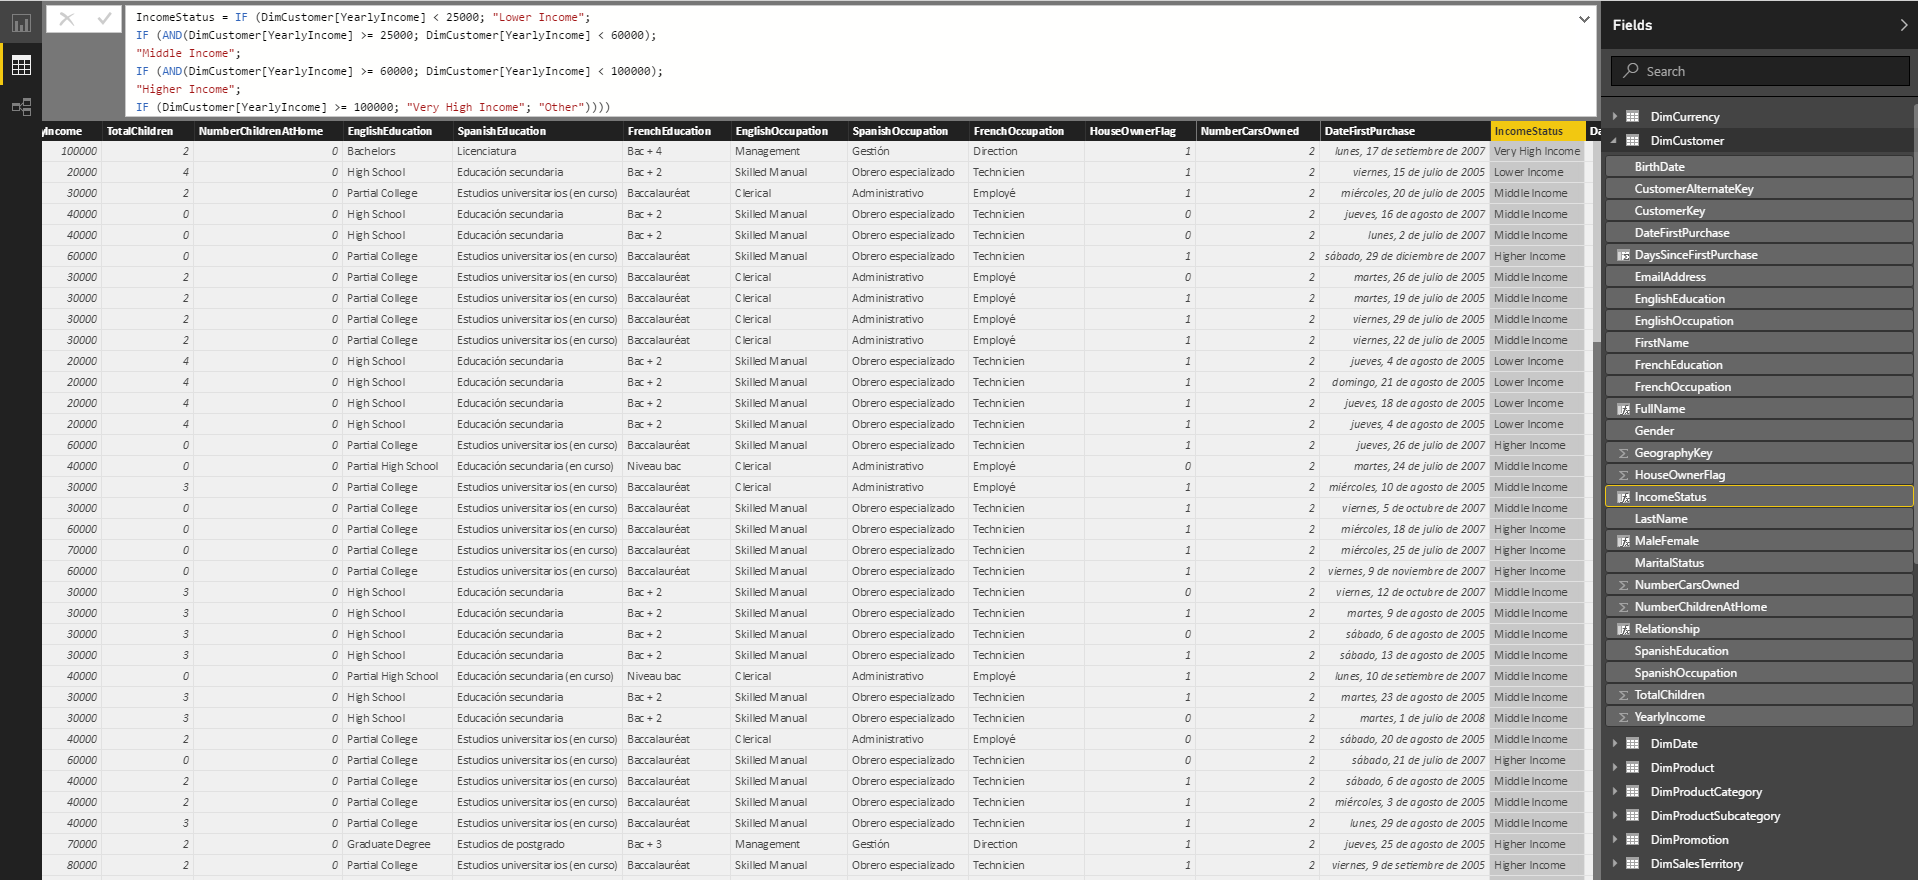
\includegraphics[width=17cm]{./Imagenes/31} 
	\end{center}

	\item  En Power BI Desktop, haga clic en Datos en el panel de vistas en el lado izquierdo. En el panel Campos, haga clic en DimCustomer.  En la cinta Modelado, en el grupo Cálculos, haga clic en Nueva columna. En la barra de fórmulas, resalte Columna = y escriba:
	\\
	\\
	\\DaysSinceFirstPurchase = DATEDIFF(DimCustomer[DateFirstPurchase], TODAY(), DAY) \\
	\\
\\
	\begin{center}
	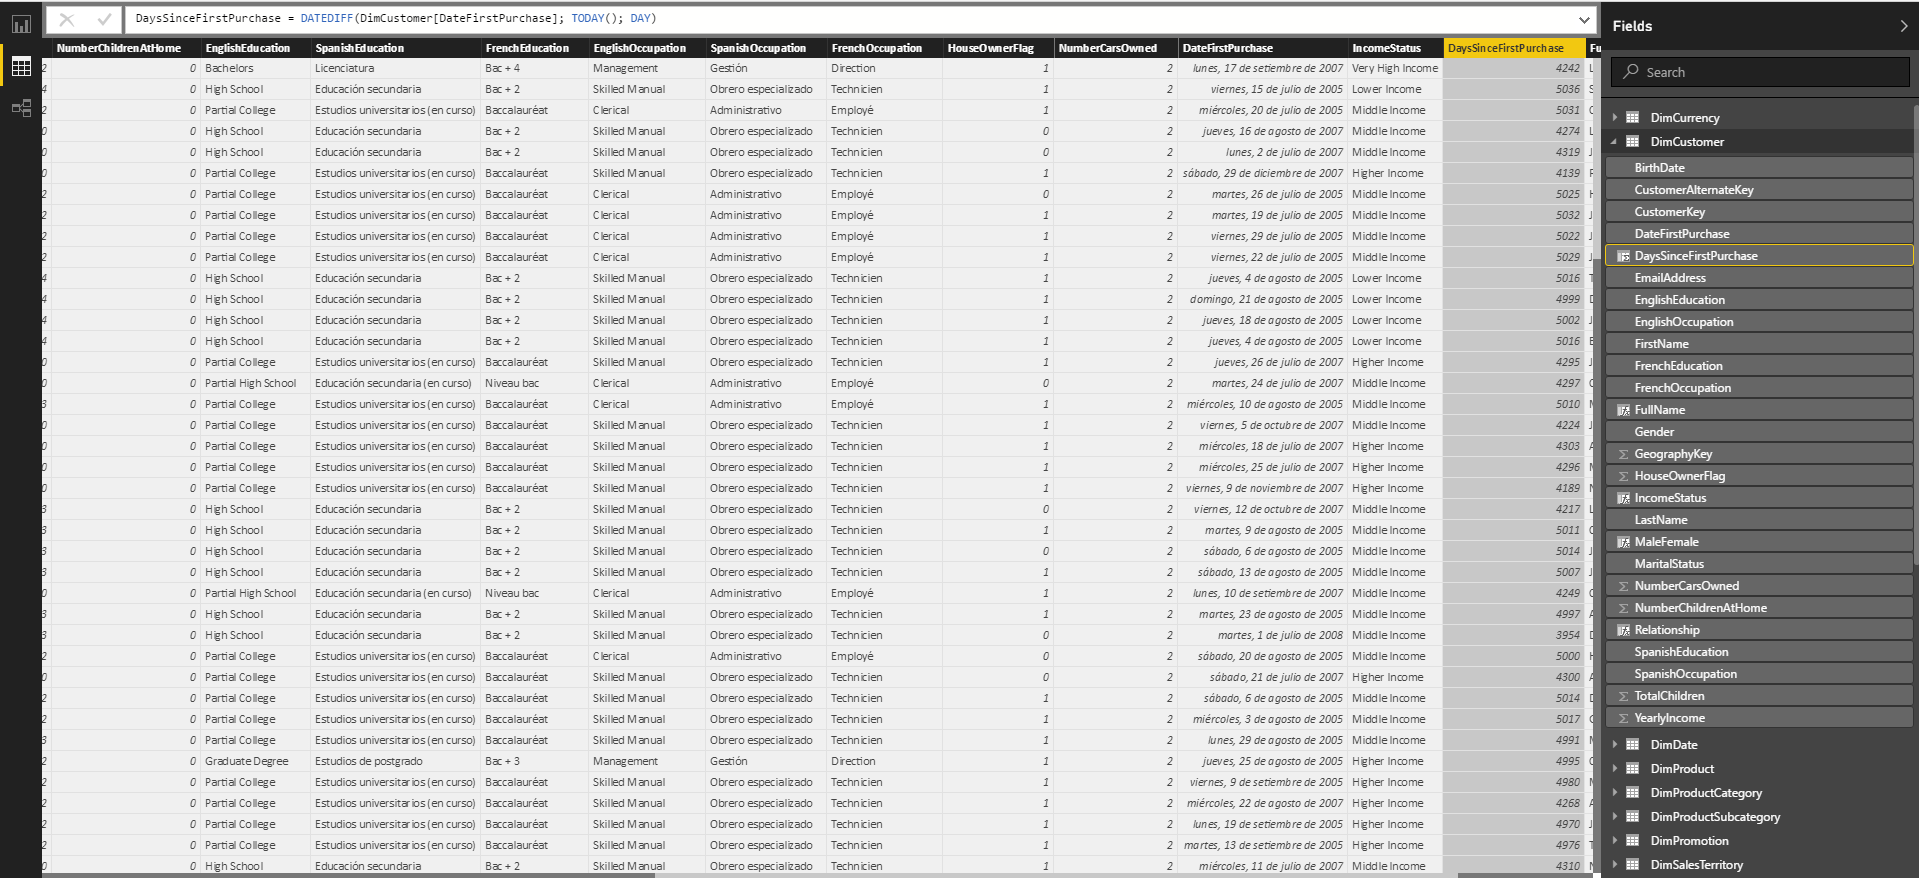
\includegraphics[width=17cm]{./Imagenes/32} 
	\end{center}


	\item En Power BI Desktop, haga clic en Datos en el panel de vistas en el lado izquierdo. En el panel Campos, haga clic en DimCustomer.  En la cinta Modelado, en el grupo Cálculos, haga clic en Nueva columna. En la barra de fórmulas, resalte Columna = y escriba:
	\\
	
			 
	\begin{center}
	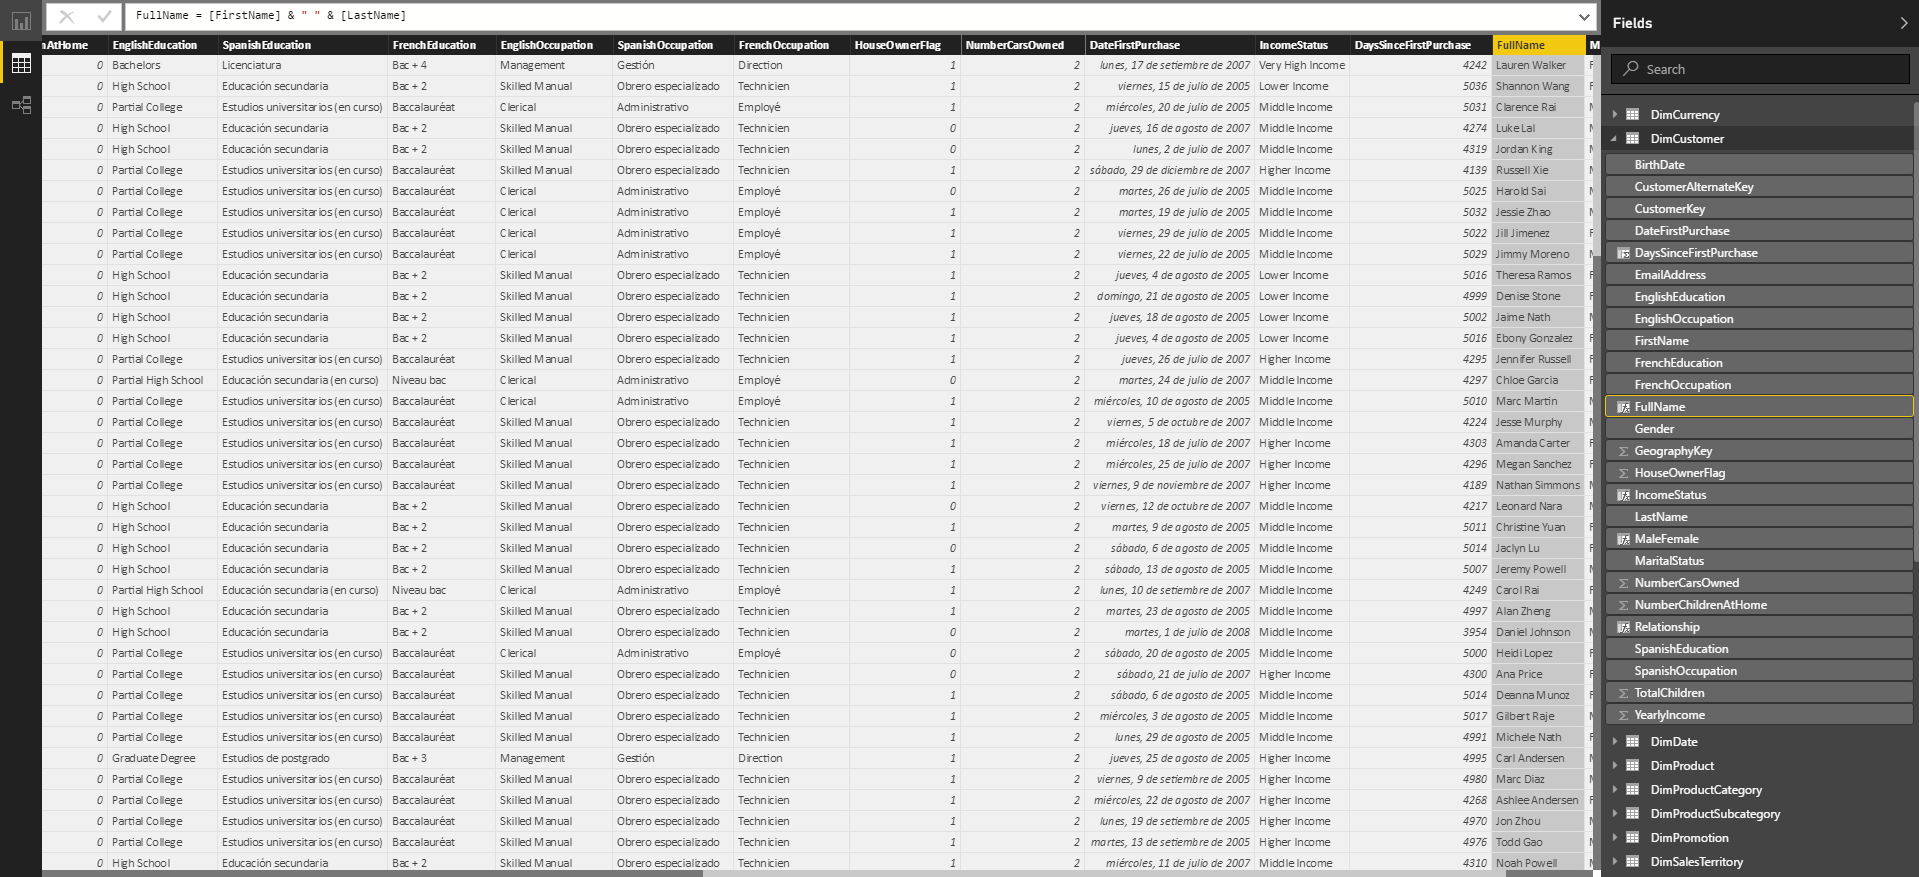
\includegraphics[width=17cm]{./Imagenes/33} 
	\end{center}


	\item En Power BI Desktop, haga clic en Datos en el panel de vistas en el lado izquierdo. En el panel Campos, haga clic en DimCustomer.  En la cinta Modelado, en el grupo Cálculos, haga clic en Nueva columna. En la barra de fórmulas, resalte Columna = y escriba:
	\\
	\\MaleFemale = IF([Gender] = "M", "Male", "Female")\\
			 
	\begin{center}
	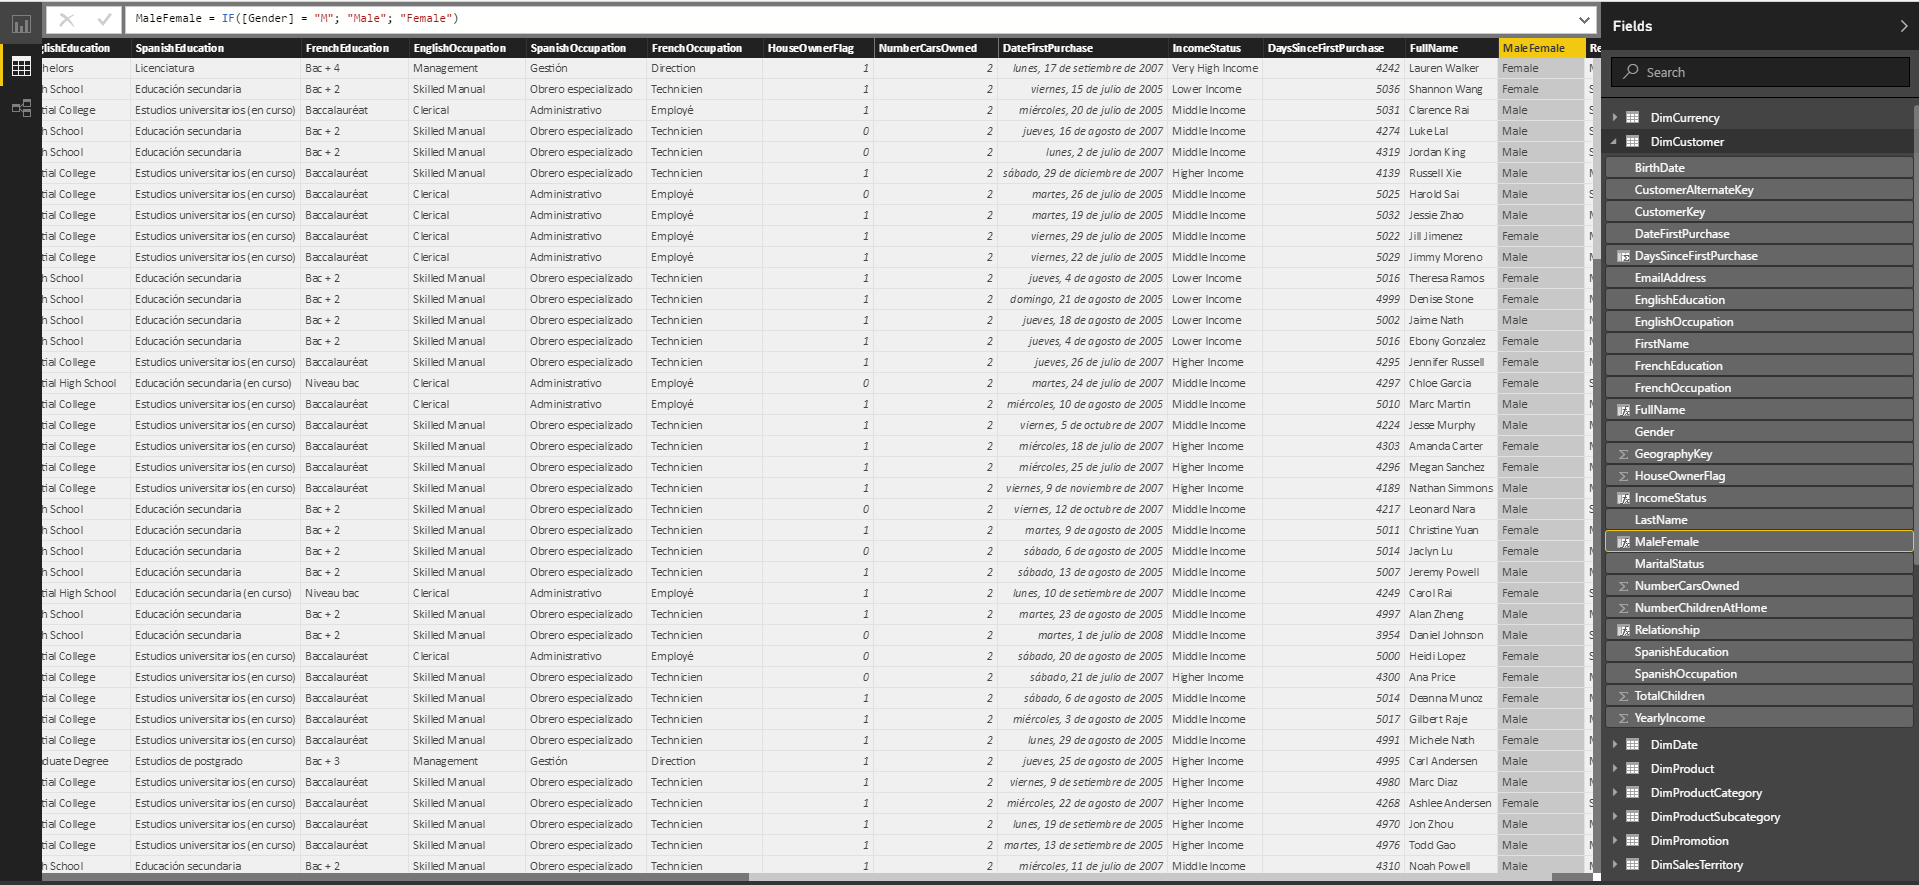
\includegraphics[width=17cm]{./Imagenes/34} 
	\end{center}

	\item En Power BI Desktop, haga clic en Datos en el panel de vistas en el lado izquierdo. En el panel Campos, haga clic en DimCustomer.  En la cinta Modelado, en el grupo Cálculos, haga clic en Nueva columna. En la barra de fórmulas, resalte Columna = y escriba:
	\\
	\\Relationship = IF([MaritalStatus] = "M", "Married", "Single")\\
			 
	\begin{center}
	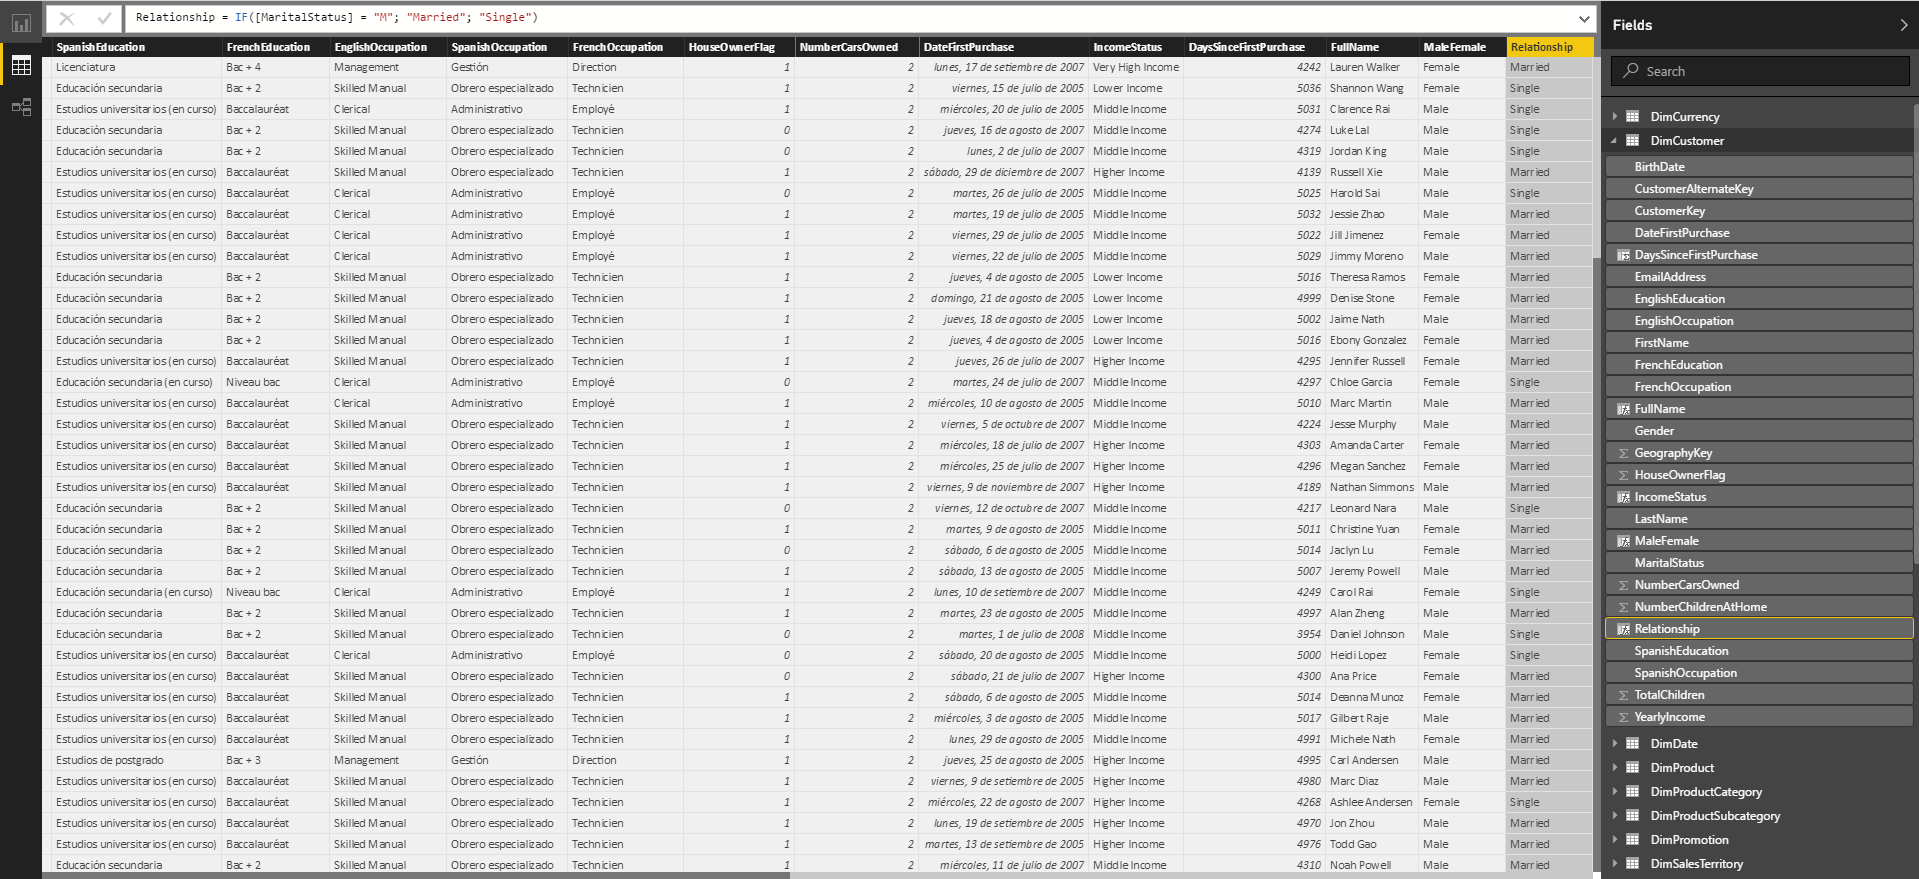
\includegraphics[width=17cm]{./Imagenes/35} 
	\end{center}

	\item En Power BI Desktop, haga clic en Datos en el panel de vistas en el lado izquierdo. En el panel Campos, haga clic en DimCustomer.  En la cinta Modelado, en el grupo Cálculos, haga clic en Nueva columna. En la barra de fórmulas, resalte Columna = y escriba:
	\\
	\\MainCategory = RELATED(DimProductCategory[CategoryName])\\
			 
	\begin{center}
	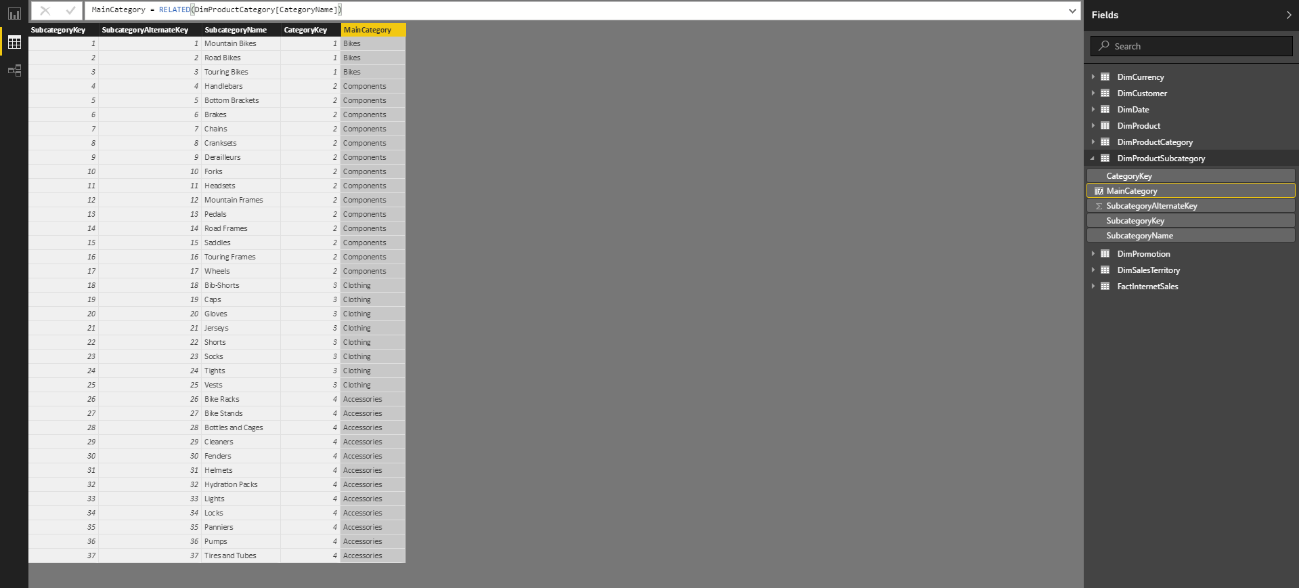
\includegraphics[width=17cm]{./Imagenes/36} 
	\end{center}

	\item En Power BI Desktop, haga clic en Datos en el panel de vistas en el lado izquierdo. En el panel Campos, haga clic en DimPromotion.  En la cinta Modelado, en el grupo Cálculos, haga clic en Nueva columna. En la barra de fórmulas, resalte Columna = y escriba:
	\\
	\\PromotionLengthDays = DATEDIFF(DimPromotion[StartDate], DimPromotion[EndDate], DAY)\\
			 
	\begin{center}
	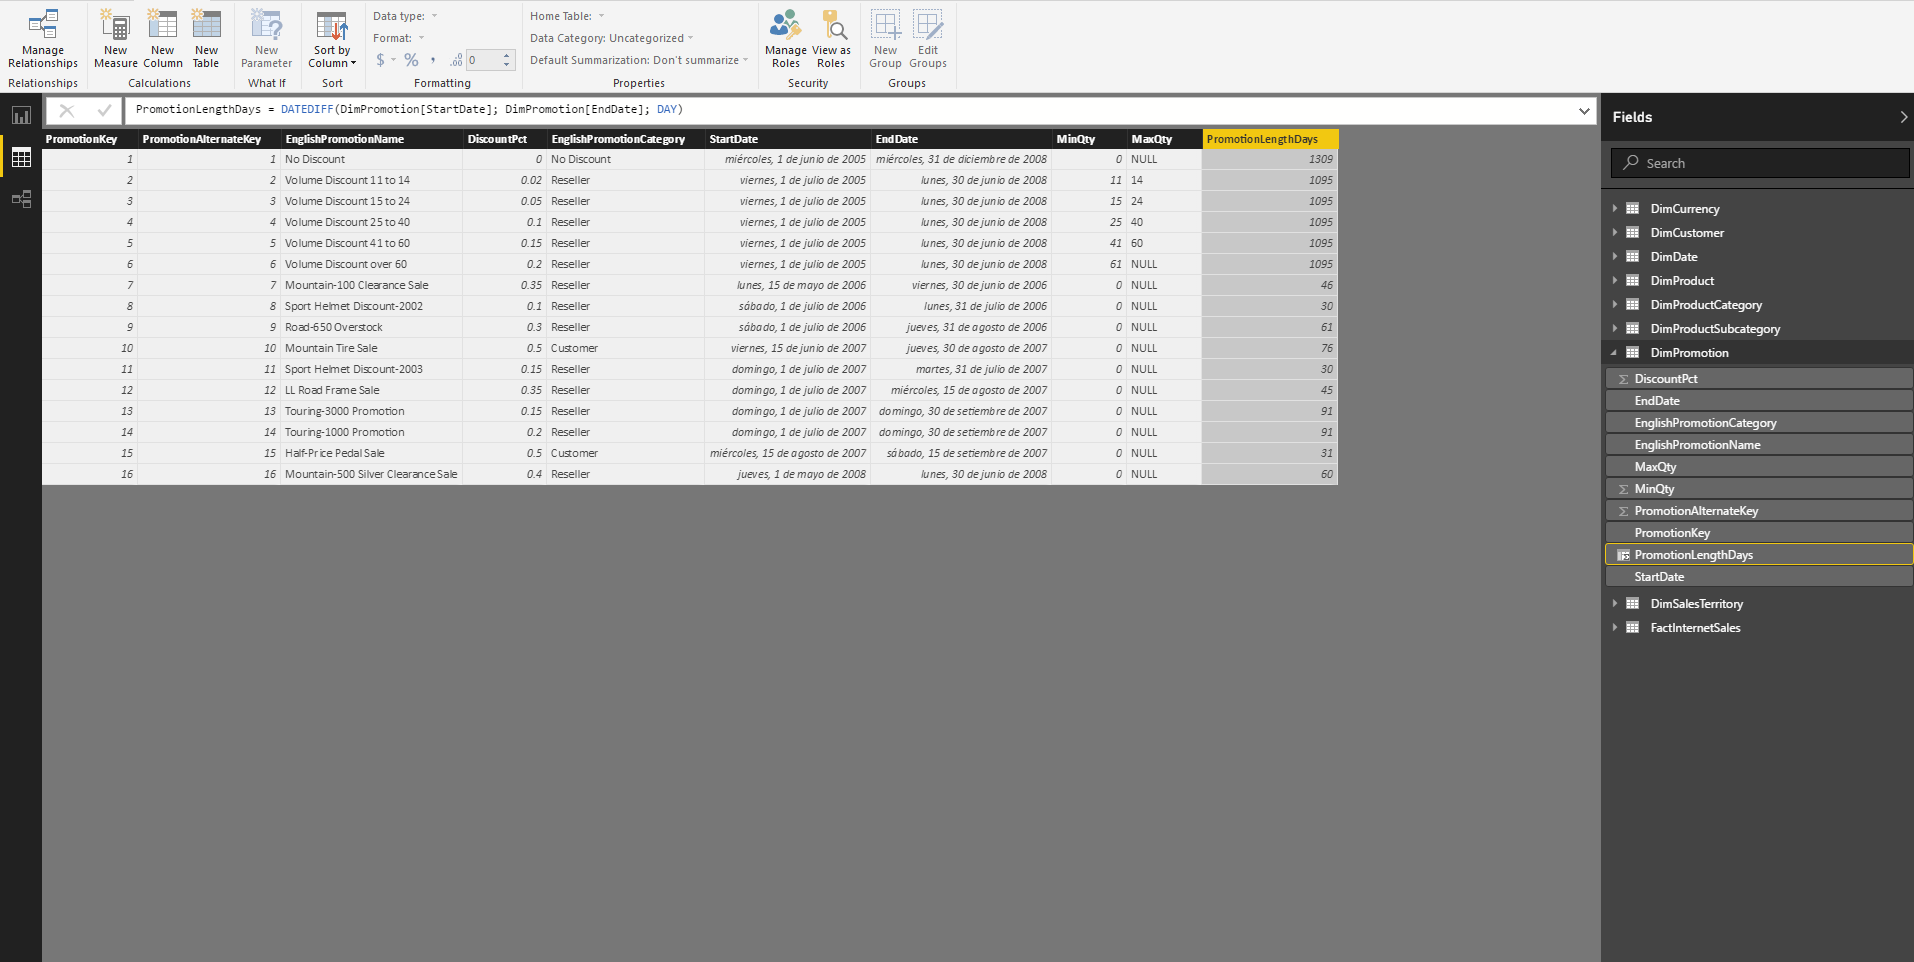
\includegraphics[width=17cm]{./Imagenes/37} 
	\end{center}


	\item En Power BI Desktop, haga clic en Datos en el panel de vistas en el lado izquierdo. En el panel Campos, haga clic en DimPromotion.  En la cinta Modelado, en el grupo Cálculos, haga clic en Nueva columna. En la barra de fórmulas, resalte Columna = y escriba:
	\\
	\\Profit = CURRENCY(FactInternetSales[UnitPrice] - \\
FactInternetSales[ProductStandardCost])\\
			 
	\begin{center}
	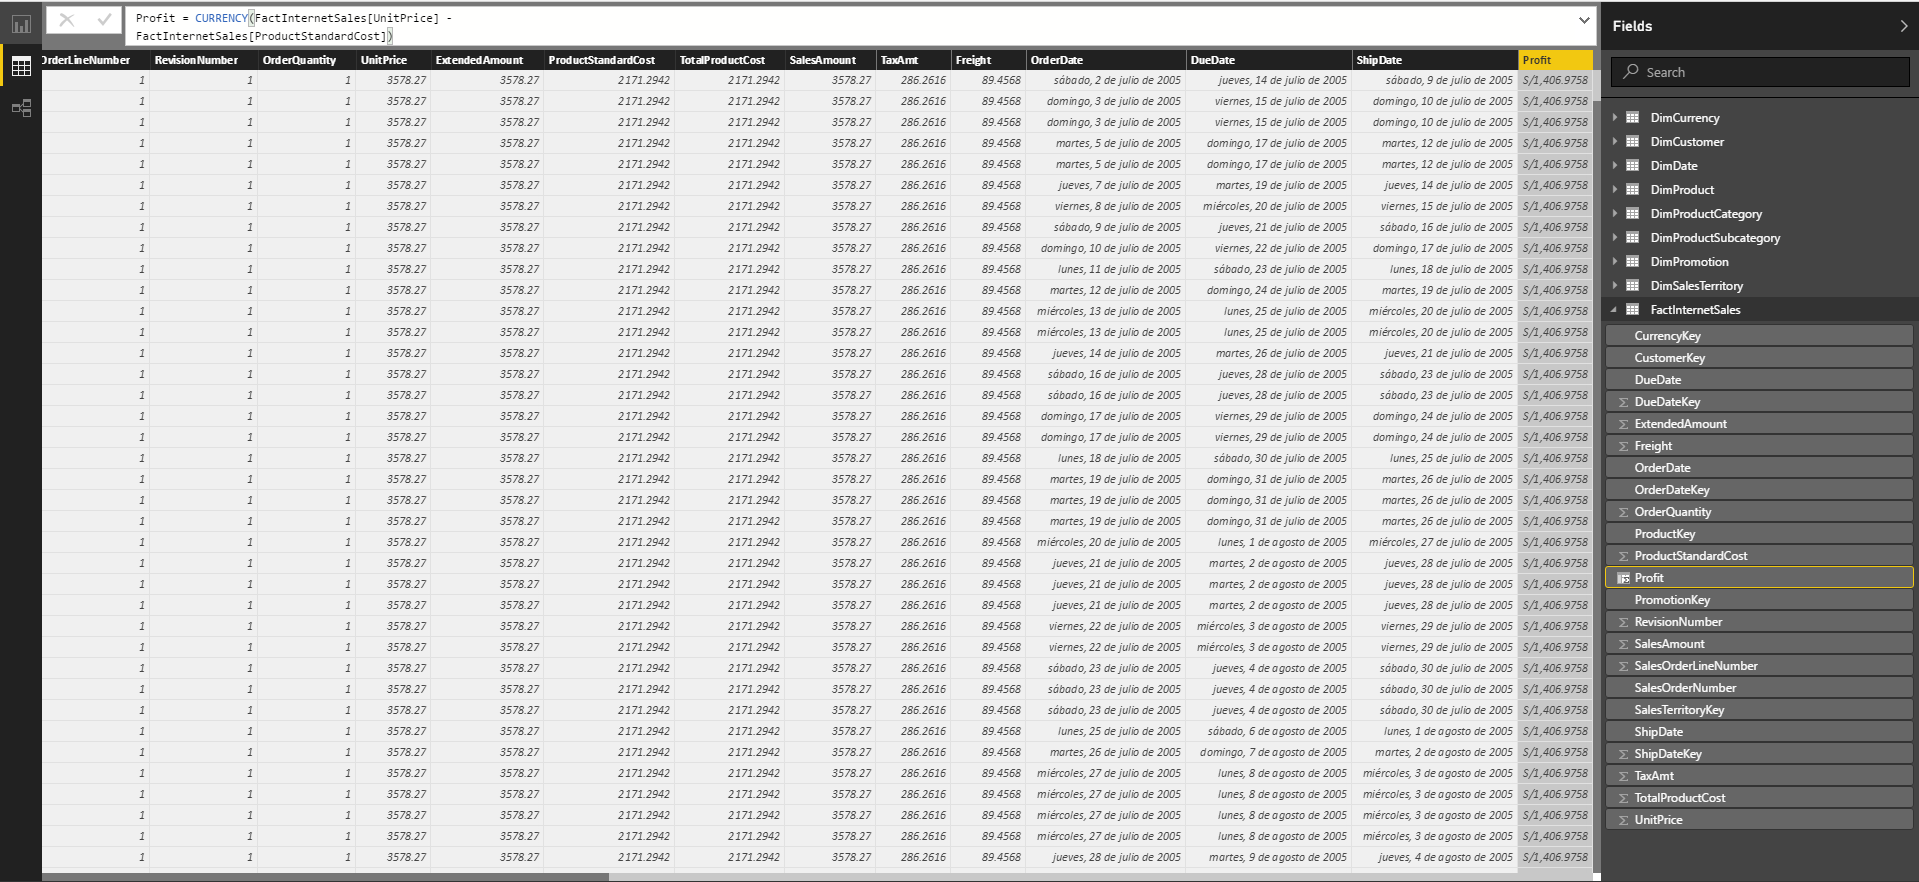
\includegraphics[width=17cm]{./Imagenes/38} 
	\end{center}

\end{enumerate}



